\documentclass[conference,10pt,letterpaper]{IEEEtran}
\IEEEoverridecommandlockouts
% The preceding line is only needed to identify funding in the first footnote. If that is unneeded, please comment it out.
\usepackage{cite}
\usepackage{amsmath,amssymb,amsfonts}
\usepackage{algorithmic}
\usepackage{graphicx}
\usepackage{textcomp}
\usepackage{xcolor}
\usepackage{fancyhdr}
\usepackage[hidelinks]{hyperref} % Include this package to use hyperlinks
\usepackage{stfloats}
\usepackage{ulem}
\usepackage{array}
\usepackage{amssymb} % for \checkmark
\usepackage{tabularx} % for width-adjustable tables
\usepackage{booktabs} % for better line separators
\usepackage{color}

% Set single spacing
\linespread{1}

% Times New Roman font (if required, uncomment the next line)
\usepackage{times}

\def\BibTeX{{\rm B\kern-.05em{\sc i\kern-.025em b}\kern-.08em
		T\kern-.1667em\lower.7ex\hbox{E}\kern-.125emX}}
	
%\setlength{\parindent}{0pt}	

\begin{document}
	
	\title{Wattson: An Innovative IELTS Speaking Assistant Android Application}
	
	% Ensure that all author blocks are centered and on the same line
	\makeatletter
	\newcommand{\authorblock}[2]{
		\parbox[t]{.3333\textwidth}{\centering #1\\#2}
	}
	\makeatother
	
	\author{
		\authorblock{Kaijie Lai}{
			2034675\\
			\href{mailto:Kaijie.Lai20@student.xjtlu.edu.cn}{Kaijie.Lai20@student.xjtlu.edu.cn}
		}
		\authorblock{Zhen Ma}{
			2034590\\
			\href{mailto:Zhen.Ma20@student.xjtlu.edu.cn}{Zhen.Ma20@student.xjtlu.edu.cn}
		}
		\authorblock{Jinxing Li}{
			20XXXXX\\
			\href{mailto:Jinxing.Li20@student.xjtlu.edu.cn}{Jinxing.Li20@student.xjtlu.edu.cn}
		}\\ \\[10pt]
		\authorblock{Yichen Liang}{
			20XXXXX\\
			\href{mailto:Yichen.Liang20@student.xjtlu.edu.cn}{Yichen.Liang20@student.xjtlu.edu.cn}
		}
		\authorblock{Keming Shen}{
			20XXXXX\\
			\href{mailto:Keming.Shen20@student.xjtlu.edu.cn}{Keming.Shen20@student.xjtlu.edu.cn}
		}
	}

	\maketitle
	
	\thispagestyle{fancy}
	
	%header
	\pagestyle{fancy} % This sets the fancy style for all pages
	\fancyhead[LO,L]{CAN 301}
	\fancyhead[CO,C]{Mobile Computing}
	\fancyhead[RO,R]{\today}
	\fancyfoot[LO,L]{}
	\fancyfoot[CO,C]{\thepage}
	\fancyfoot[RO,R]{}
	\renewcommand{\headrulewidth}{0.4pt}
	\renewcommand{\footrulewidth}{0.4pt}
	
	\section{Introduction}
	This report presents development and evaluation of "Wattson", an innovative IELTS Speaking Assistant Android application designed to aid students in IELTS speaking practice. The report details the app design, including its user interface and functional features, followed by an evaluation of its effectiveness in aiding IELTS speaking preparation. 
	
	\subsection{Motivation}
	
	\begin{table*}[b]
		\centering
		\caption{Comparative Analysis of IELTS Preparation Apps}
		\label{tab:my-table}
		\begin{tabularx}{\textwidth}{@{}l *{6}{X} c@{}} % Adjust the number of X's based on your column count
			\toprule
			\textbf{APP} & \textbf{Question Library} & \textbf{Simulate Exam} & \textbf{Pronunciation Practice} & \textbf{Playback} & \textbf{Random Question} & \textbf{Note \& Record Storage} \\
			\midrule
			Wattson                & \checkmark & & & \checkmark & \checkmark & \checkmark \\
			China Daily            & & & \checkmark & & & \\
			Duolingo               & & & \checkmark & & & \\
			Minor Station IELTS    & \checkmark & \checkmark & & \checkmark & & \\
			IELTS Official Pre App & \checkmark & \checkmark & & \checkmark & \checkmark & \\
			Simon IELTS            & \checkmark & \checkmark & & & \checkmark & \\
			\bottomrule
		\end{tabularx}
	\end{table*}
	
	For more than three decades, the International English Language Testing System (IELTS) has been a pivotal benchmark in assessing English language proficiency, trusted by over 12,000 institutions in approximately 140 nations. However, a significant challenge has been identified in the context of Chinese students' performance in the IELTS Speaking section. This challenge does not stem from a fundamental deficiency in English proficiency but rather from a critical shortfall in effective and practical oral language training.
	
	As a student at Xi'an Jiaotong-Liverpool University, where many aspire to pursue postgraduate studies abroad, proficiency in the IELTS exam, particularly in the speaking part, is a common requirement. In my personal experience and observations, achieving a high score in the IELTS Speaking section necessitates repetitive practice and training, but students often struggle with rigid, rehearsed responses and lack the adaptability essential for genuine linguistic advancement.
	
	Recognizing the inefficiency of traditional practice methods, which involve a cumbersome process of operating a recorder and managing speaking prompts, we were motivated to develop an innovative IELTS speaking practice application. This application aims to streamline the IELTS speaking practice by integrating a database of questions with an easy-to-use recording feature, allowing users to focus on enhancing their speaking skills without the hassle of juggling multiple devices or applications.
	
	Our project is propelled by a dual commitment: firstly, to tackle specific obstacles encountered by Chinese learners in the Speaking section, and secondly, to make IELTS preparation more accessible and financially viable. Current software solutions in the market, such as voice assistant apps, lack targeted training features and do not address the need for structured and practical oral language training.
	
	This initiative is not merely an endeavor to enhance test scores but a strategic effort to bridge a critical educational gap. By facilitating a more comprehensive and practical approach to mastering the spoken aspect of the English language, we aim to ensure that economic limitations do not obstruct individuals' journey towards English language mastery.
	
	\subsection{Contribution}
	
	\begin{figure*}[ht]
		\centering
		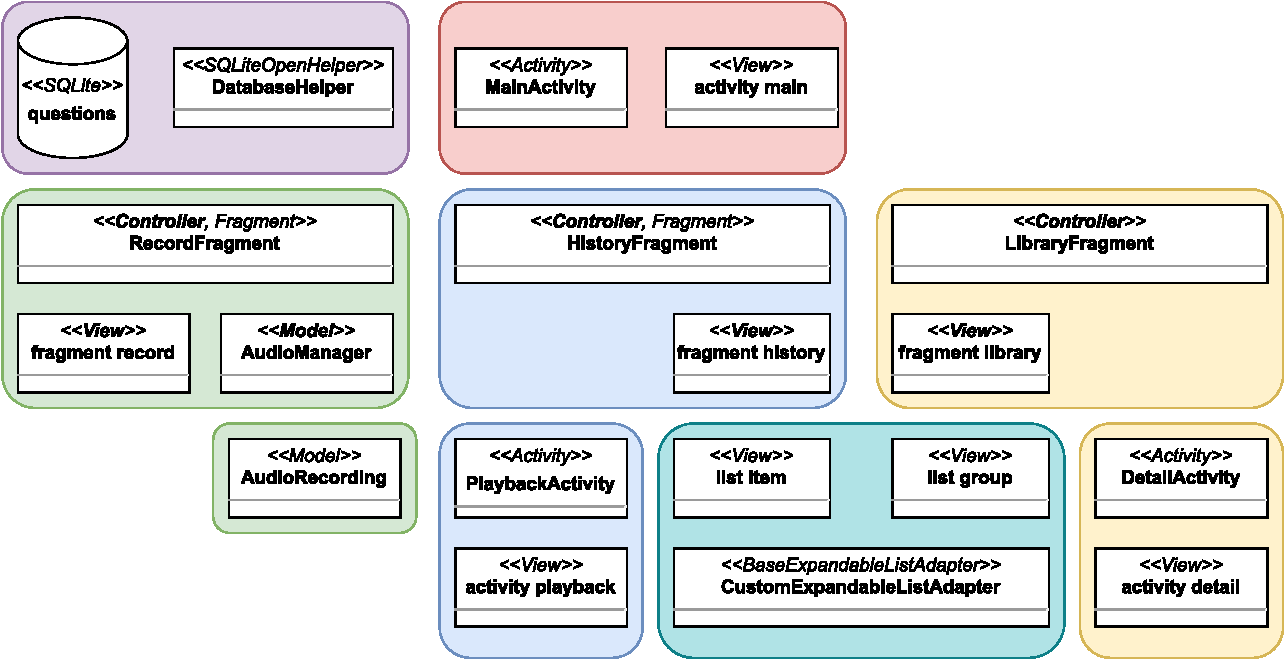
\includegraphics[width=6.2in]{src/all-classes.pdf}
		\caption{MVC Architecture of Project}
		\label{fig:all_classes}
	\end{figure*}
	
	Incorporating the emphasis on adherence to the Model-View-Controller (MVC) architecture into the description of the IELTS Speaking Practice Application, the revised content is as follows:
	
	\newpage
	The Wattson offers a tailored platform for IELTS candidates, particularly focused on the speaking section of the test. Our application is designed following the strict principles of the Model-View-Controller (MVC) architecture, as depicted in Figure \ref{fig:all_classes}. This architectural approach enhances learning through realistic simulation and immediate feedback via recording features, providing a user-friendly experience that allows for personalized practice sessions. Its convenience, clarity, and structured approach to organizing study materials, aligned with the MVC model, significantly contribute to a user's ability to improve their speaking skills efficiently, making it a valuable tool in the IELTS preparation process.
	
	A comparative analysis of existing market offerings was conducted to identify gaps in current applications and guide the development of our app. This analysis, summarized in a comparative table, revealed that popular applications like 'China Daily' and 'Duolingo' lack specialized features for IELTS Speaking Test preparation, such as a dedicated IELTS test bank and exam simulation. These applications predominantly focus on general speaking practice, omitting IELTS-specific content. Moreover, while other applications possess a broader range of functionalities, they exhibit notable usability issues.
	
	Key issues identified in existing applications include disorganized question bank functionalities, which impede users' ability to efficiently categorize questions by parts of the speaking test. This disorganization complicates the process of locating specific questions for targeted practice. Additionally, the recording function in these apps does not permit users to save their recordings. Consequently, if a user exits the exam page, they lose access to previous recordings, hindering their ability to review and refine their speaking skills.
	
	Our application, adhering to the MVC architecture, addresses these shortcomings by offering streamlined access to the question bank, enabling users to filter questions by test part swiftly. This feature significantly enhances both the efficiency and the user experience. Furthermore, our app's capability to save, edit, and retrieve historical recording records fills a critical gap in the market, addressing the limitations of existing applications that do not support recording preservation.
	
	In summary, our IELTS Speaking Practice Application is distinctively positioned to cater to the specific needs of IELTS test takers. By offering tailored functionalities for IELTS Speaking Test preparation, within the MVC framework, our app provides a convenient and effective platform for users to practice and enhance their skills anytime and anywhere. These user-centric features, coupled with our adherence to the MVC architecture, are pivotal in attracting and retaining our user base.
	
	\section{App Design}
	
	In this section, we delve into the intricacies of two primary features of our application: the Record feature and the Bottom Navigation. These features are dissected from multiple perspectives to provide a comprehensive understanding of their design and functionality.
	
	\subsection{Record Feature}
	The Record feature is a crucial component of the app, and its design is considered from the following aspects:
	
	\begin{figure}[htbp]
		\centerline{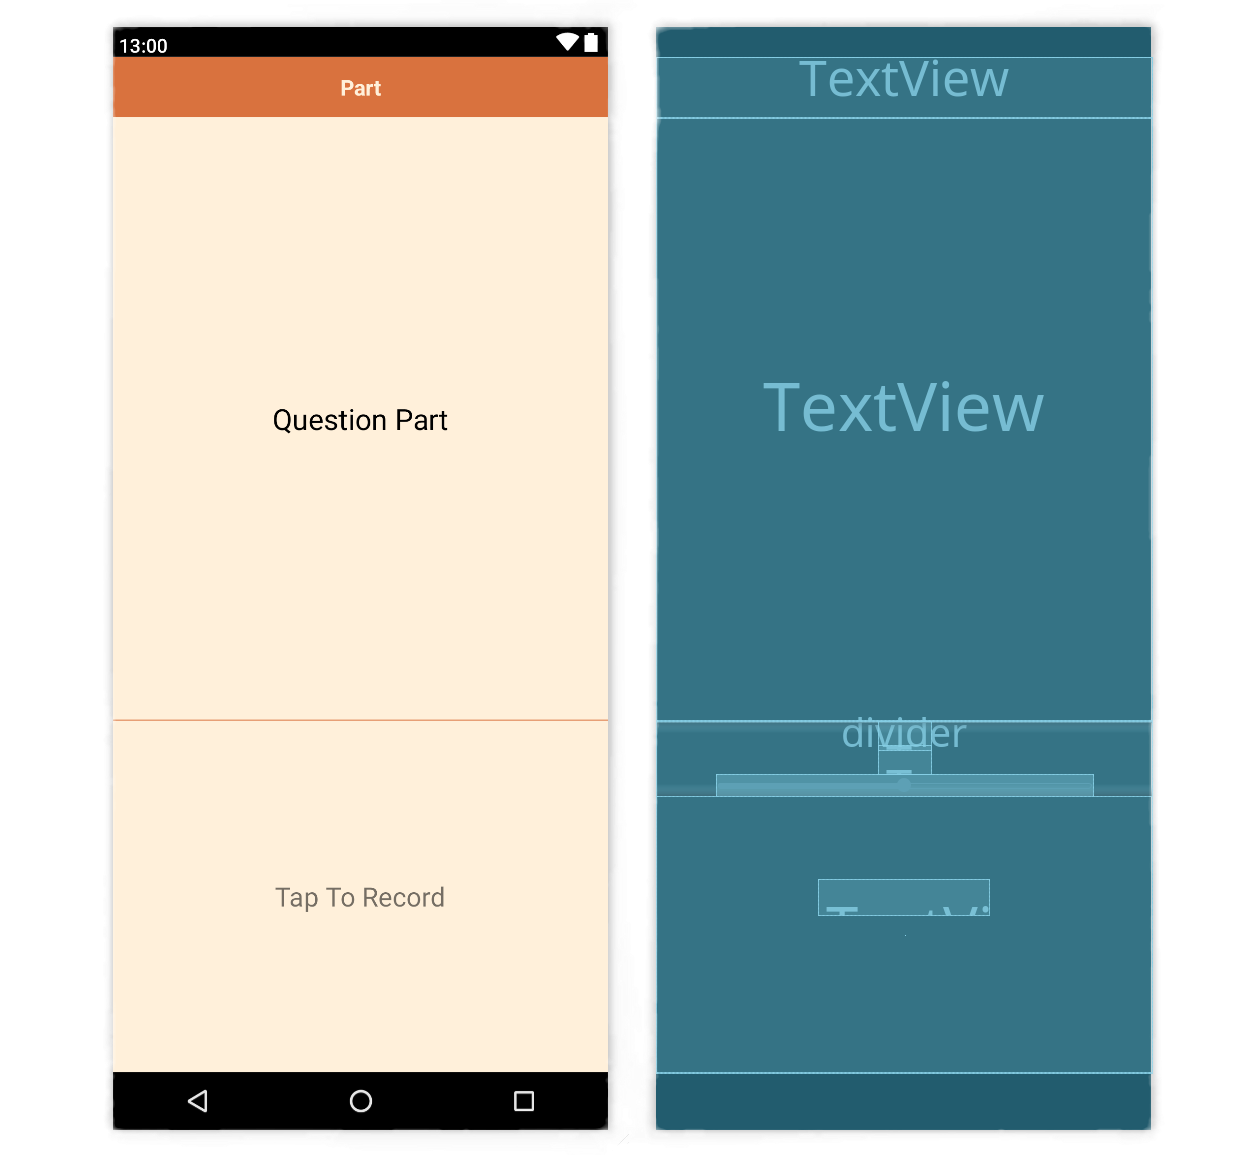
\includegraphics[width=\columnwidth]{src/record layout remove.png}}
		\caption{Layout View of Record Fragment}
		\label{fig:record_layout}
	\end{figure}
	
	\begin{figure}[htbp]
		\centerline{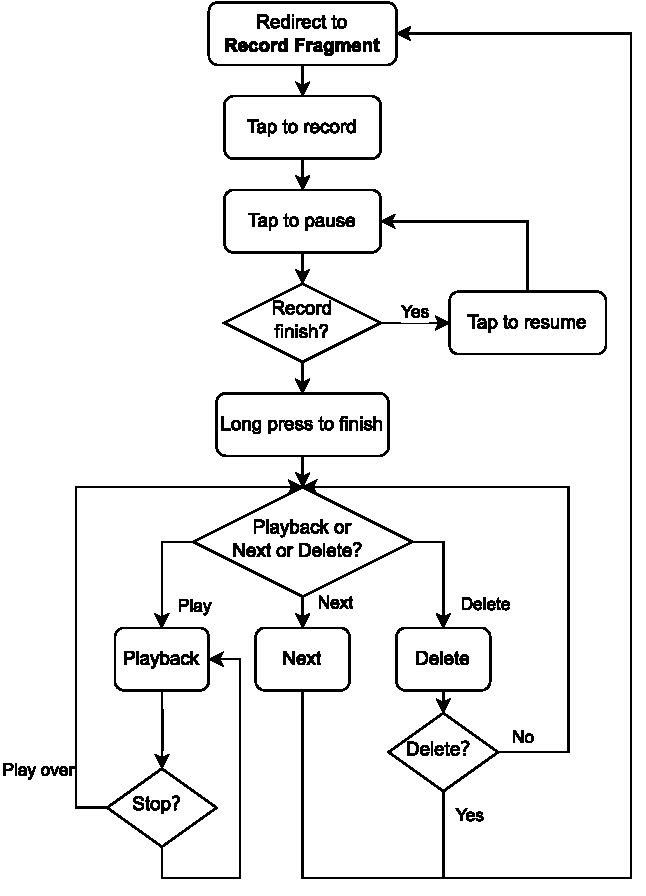
\includegraphics[width=3.1in]{src/flowchart.pdf}}
		\caption{Flowchart of Record Instruction}
		\label{fig:flowhart}
	\end{figure}
	
	\begin{itemize}
		\item \textbf{User Interface (UI)}: 
		The primary components of the View for the Record feature are defined in the \texttt{res/layout/fragment\_record.xml}. The corresponding class diagram illustrates the object structure in Figure \ref{fig:record_part}. Initially, the UI layout is as shown in the schematic Figure \ref{fig:record_layout}. Interaction and visibility of different UI elements, such as buttons, are controlled in \texttt{RecordFragment} by modifying their visibility attributes (visible, invisible, or gone). The View utilizes components like \texttt{TextView}, \texttt{View}, \texttt{SeekBar}, and \texttt{ImageButton}, while the ViewGroup includes \texttt{FrameLayout}, \texttt{LinearLayout}, and \texttt{GridLayout}. The app's theme, set in \texttt{values/themes/themes.xml}, employs a \texttt{NoActionBar} style for a clean interface without a primary bar. Colors used throughout the application are defined in \texttt{values/colors.xml}, and all fundamental strings are set in \texttt{values/strings.xml}.
		
		\begin{figure}[htbp]
			\centerline{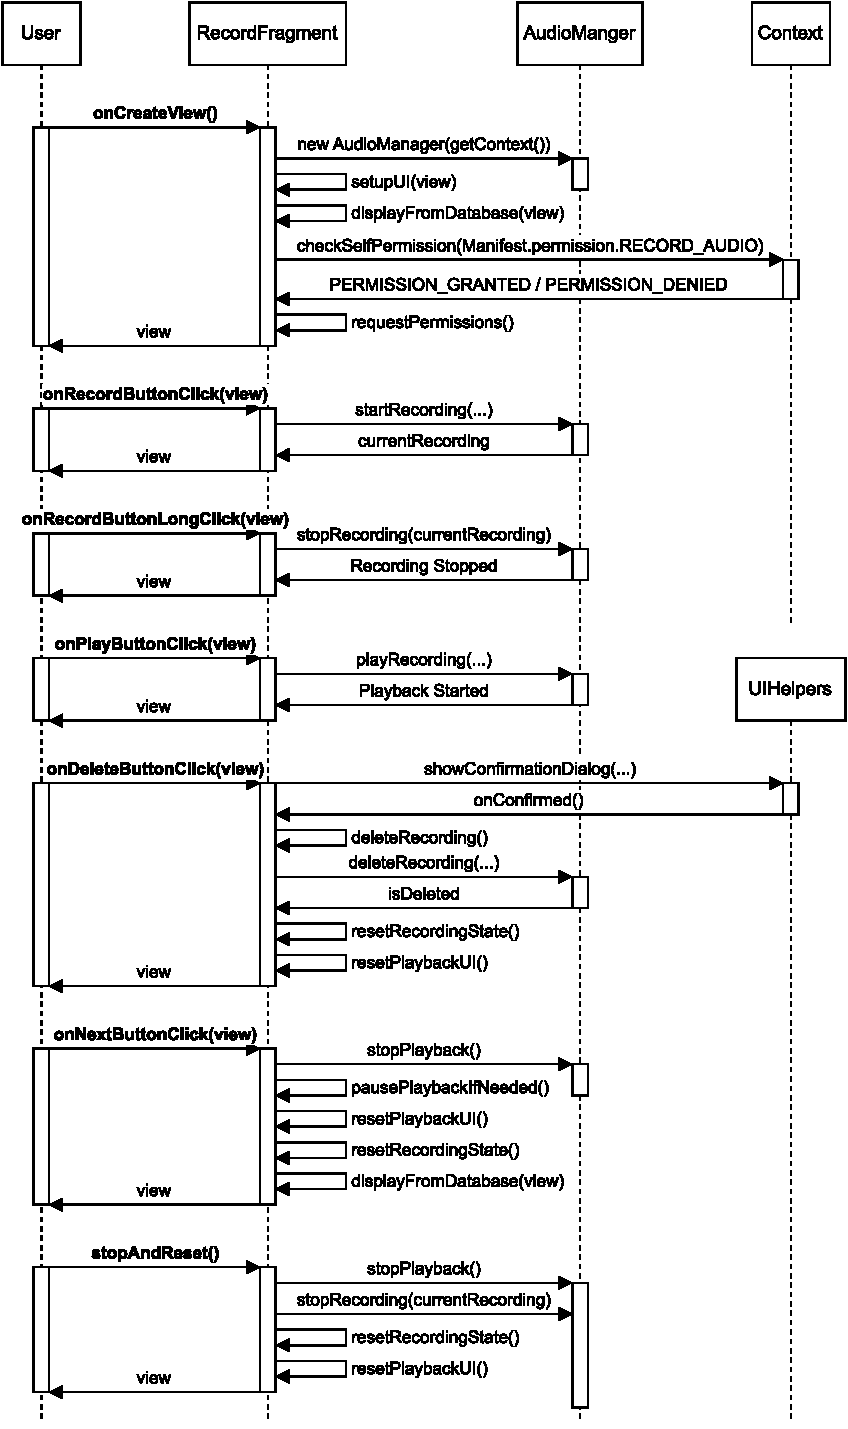
\includegraphics[width=\columnwidth]{src/record-sequence.pdf}}
			\caption{Sequence Diagram of RecordFragment}
			\label{fig:record_sequence}
		\end{figure}
		
		\item \textbf{User Experience (UX)}: 
		Upon opening the app, users are automatically directed to the Record Part (as shown in the attached Figure \ref{fig:record_part}). At the top of the page, users see a question from the database along with its corresponding Part. Following the prompt \texttt{Tap to record} begins the recording process. A subsequent tap changes the prompt to \texttt{Tap to pause}, allowing users to pause the recording. Options then include \texttt{Tap to resume} or \texttt{Long press to finish}. After recording, users can see their recording with options to play it back by pressing the play button and navigate through the recording using the progress bar. The \texttt{Next} button allows users to proceed to the next question, saving the current recording. If unsatisfied, the \texttt{Delete} option is available to remove the recording, accompanied by a system prompt for confirmation and a toast message \texttt{Recording deleted successfully} upon deletion. This workflow constitutes the entire user experience of the Record functionality in the flowchart Figure \ref{fig:flowhart}.
		
		\begin{figure*}
			\centering
			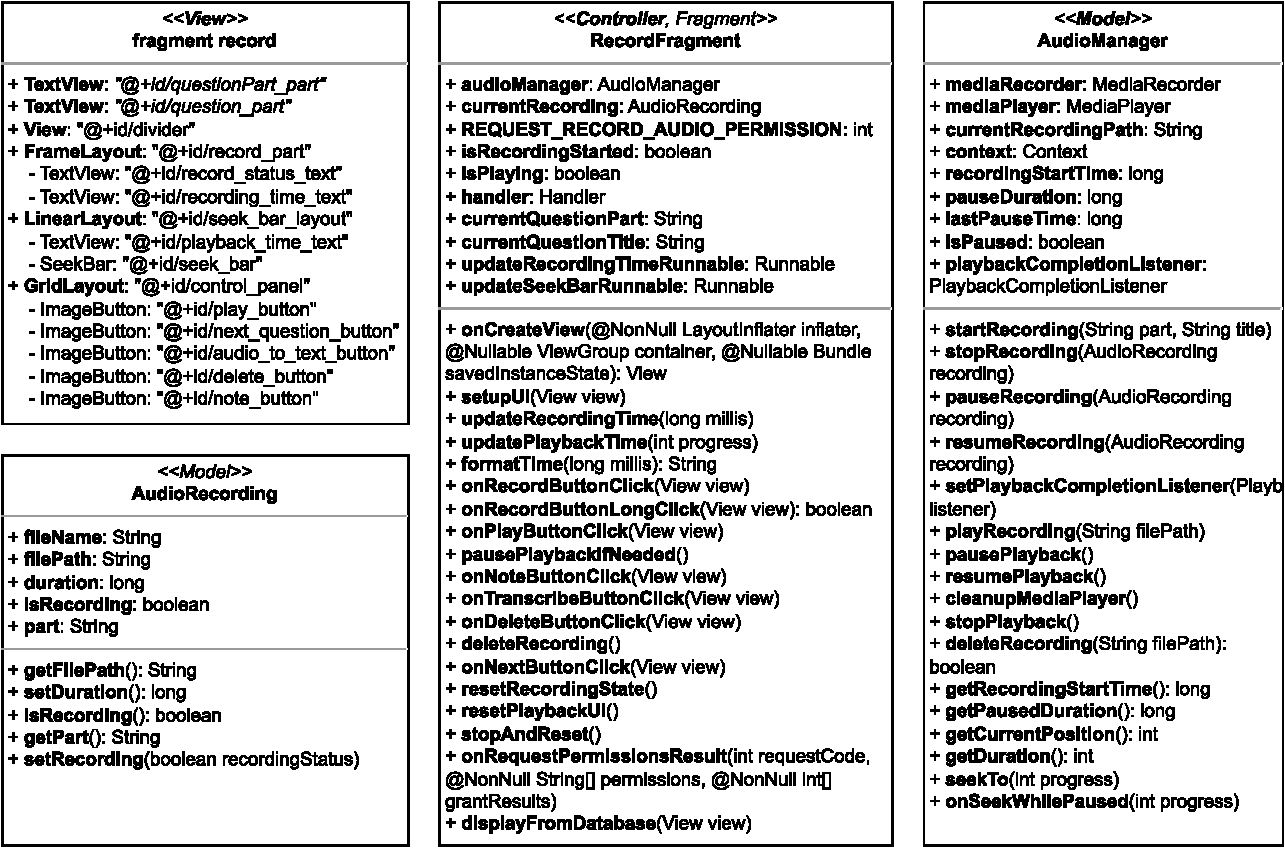
\includegraphics[width=6.2in]{src/record part.pdf}
			\caption{Classes Diagram of Record Part}
			\label{fig:record_part}
		\end{figure*}
		
		\item \textbf{Permissions and Data Management}: 
		The class of \texttt{RecordFragment} manages permissions and data intricately. It checks for audio recording permissions using the \texttt{ContextCompat.checkSelfPermission} method and requests them if not already granted. This ensures that the app adheres to Android's security norms. Additionally, the class interacts with the \texttt{DatabaseHelper} like in Figure \ref{fig:datahelper} to retrieve and display questions from the database. This involves fetching random questions and their corresponding details, demonstrating the app's ability to manage and utilize data effectively. The management of audio files, such as creation, playback, and deletion, is handled through the \texttt{AudioManager} class, showcasing a well-structured approach to data handling and storage.
		
		\item \textbf{Error Handling and User Feedback}: 
		The code demonstrates careful consideration of error handling and user feedback. For instance, if the \texttt{Question TextView} or \texttt{Part TextView} is null, the app logs an error message, indicating a fail-safe approach to null pointer exceptions. During operations like deleting a recording, the app provides user feedback through \texttt{Toast} messages, such as "Recording deleted successfully" or "Failed to delete recording", enhancing the user experience. The use of confirmation dialogs before deleting recordings is another example of thoughtful user interaction design. Moreover, the app logs various actions and errors, such as in \texttt{displayFromDatabase} and \texttt{onDeleteButtonClick} methods, which aids in troubleshooting and ensures a smooth user experience.
		
		\item \textbf{Functionality Implementation}: 
		The implementation of the Record Fragment's functionality is illustrated in the sequence diagram in Figure \ref{fig:record_sequence} shown below. This diagram clearly depicts the flow of operations within the Record Fragment, providing a visual representation of the interactions and processes involved. The sequence diagram aids in understanding the sequential steps and the logical flow of the recording feature, from initiating a recording to handling playback and user interactions.

		\newpage
		\item \textbf{Performance Considerations}: 
		The performance of the application during various stages of interaction in the Record Part is a critical aspect of the user experience. The following Table \ref{tab:performance} presents a detailed analysis of the performance metrics associated with different events. These metrics include the duration of each event in milliseconds, CPU usage percentage, and memory usage in megabytes. The data provides valuable insights into the application's responsiveness and efficiency in resource utilization during key interactions such as starting and pausing recording, resuming recording, finishing recording, playback, and other functionalities. This analysis is instrumental in identifying potential areas for optimization to enhance the performance of the app.
		
	\end{itemize}
	
	\begin{table*}[ht]
		\centering
		\begin{tabularx}{6.2in}{|X|X|X|X|X|}
			\hline
			\textbf{Event} & \textbf{Stage} & \textbf{\textit{Duration (ms)}} & \textbf{\textit{CPU Usage (\%)}} & \textbf{\textit{Memory Usage (MB)}} \\ \hline
			Touch Event Press & Start Record  & \textit{51.48}  & \textit{1}            & \textit{49.2} \\ \hline
			Touch Event Press & Record Pause  & \textit{71.09}  & \textit{2}            & \textit{49.3} \\ \hline
			Touch Event Press & Resume Record & \textit{91.21}  & \textit{\textless{}1} & \textit{49.2} \\ \hline
			Touch Event Press & Record Finish & \textit{882.02} & \textit{1}            & \textit{49.1} \\ \hline
			Touch Event Press & Playback      & \textit{143.09} & \textit{\textless{}1} & \textit{49.2} \\ \hline
			Touch Event Press & Stop Playback & \textit{147.17} & \textit{\textless{}1} & \textit{49.3} \\ \hline
			Touch Event Press & Next          & \textit{142.03} & \textit{2}            & \textit{49.7} \\ \hline
			Touch Event Press & Delete        & \textit{103.32} & \textit{7}            & \textit{50.1} \\ \hline
		\end{tabularx}
		\caption{Performance Metrics for Record Part Progress}
		\label{tab:performance}
	\end{table*}
	
	\subsection{History and Library Part}
	The History and Library features are integral components of the app, designed to enhance user interaction and data management. Their design is considered from the following aspects:
	
	\begin{itemize}
		
		\item \textbf{User Interface (UI)}: 
		The UI in Figure \ref{fig:history_layout} for both the History and Library parts is primarily defined in \texttt{res/layout/fragment\_history.xml} and \texttt{res/layout/fragment\_library.xml}, respectively. These fragments utilize an \texttt{ExpandableListView} to display the data in a hierarchical manner. The custom adapter \texttt{CustomExpandableListAdapter} is employed to manage the data presentation, offering a dynamic and interactive UI experience. The \texttt{list\_group.xml} is used for displaying parts like Part1, Part2, etc., while \texttt{list\_item.xml} is responsible for presenting individual items such as titles or specific recordings under each part. This modular approach in the UI design allows for efficient data organization and enhances the user's ability to navigate through the content. The UI layout is further enhanced with XML-defined styles and themes, ensuring a consistent and visually appealing interface throughout the app.
		
		\newpage
		\item \textbf{User Experience (UX)}: 
		The History and Library features provide a seamless and intuitive user experience. In the History section, users can view and access their past recordings, grouped by parts, and interact with them through playback or deletion options. The Library section, on the other hand, presents a structured view of available titles, allowing users to explore and select items for further interaction. Both sections are designed with ease of navigation and interaction in mind, promoting an engaging and user-friendly experience.
		
		\begin{figure}[htbp]
			\centerline{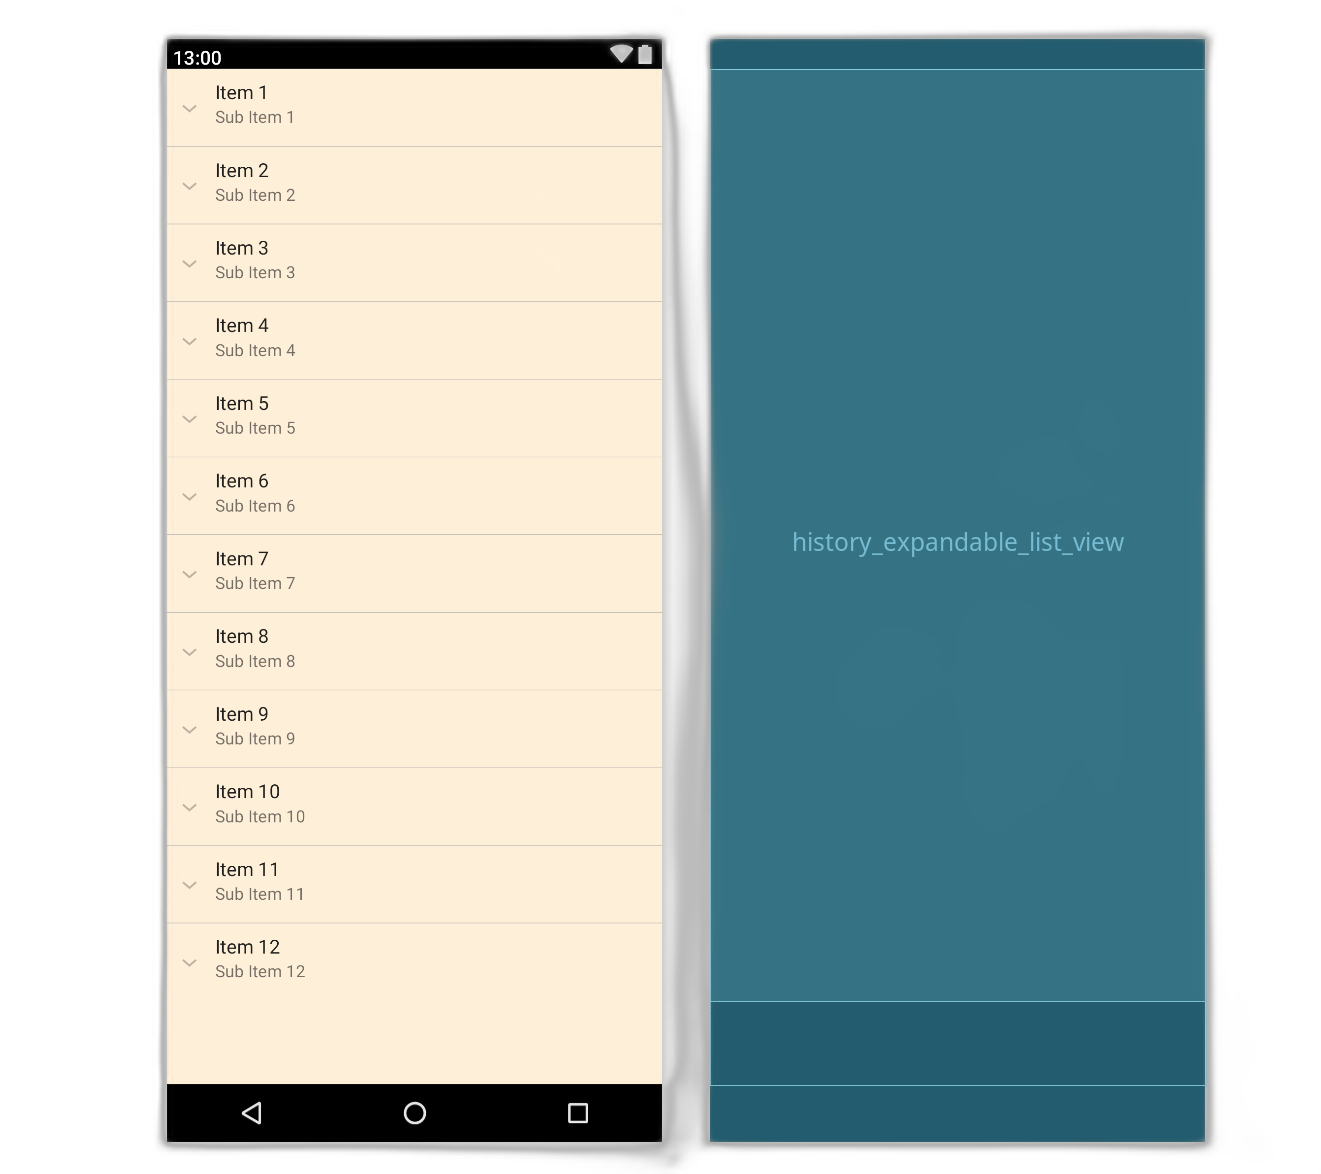
\includegraphics[width=4in]{src/history layout remove.png}}
			\caption{Layout View of Record Fragment}
			\label{fig:history_layout}
		\end{figure}
		
		\begin{figure*}[b]
			\centering
			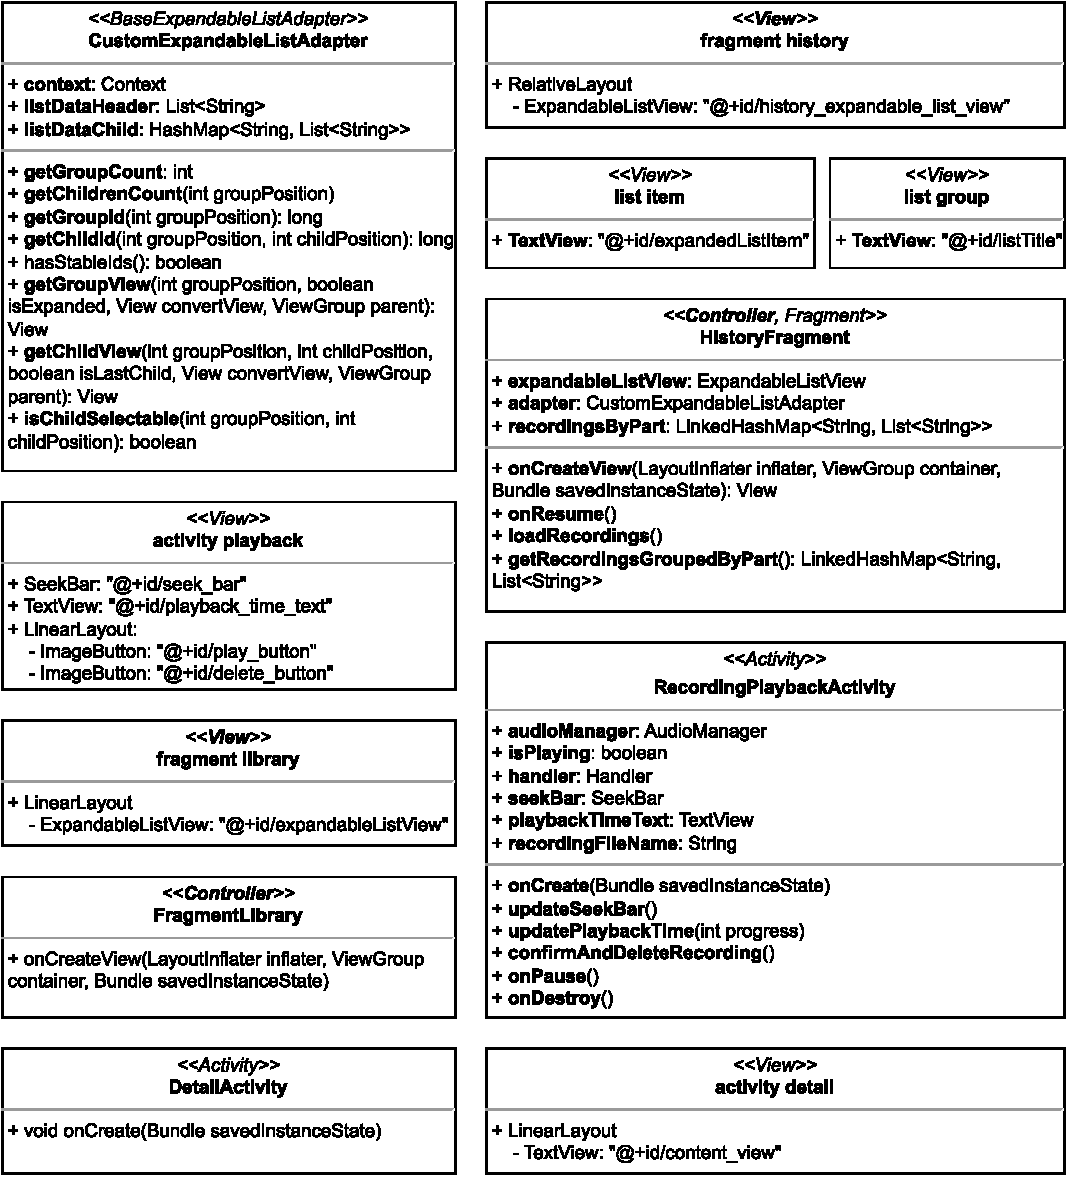
\includegraphics[width=6.2in]{src/history library part.pdf}
			\caption{Classes Diagram of Library and History Part}
			\label{fig:his_lib_classes}
		\end{figure*}
		
		
		\item \textbf{Permissions and Data Management}: 
		These features integrate smoothly with the app's data management system. In the History part, the \texttt{HistoryFragment} class manages the retrieval and display of recorded files, while the \texttt{LibraryFragment} class in the Library part interacts with the \texttt{DatabaseHelper} to fetch and display titles. This demonstrates the app's capability in handling data efficiently, ensuring a robust and responsive performance.
		
		\newpage
		\item \textbf{Error Handling and User Feedback}: 
		Both History and Library parts include prudent error handling and user feedback mechanisms. For example, if there is an issue in fetching data or accessing files, the app provides informative feedback to the user through \texttt{Toast} messages or logs. This approach not only enhances the user experience but also aids in maintaining app stability.
		
		\item \textbf{Functionality Implementation}: 
		The History and Library features' implementation can be understood through the key functions in \texttt{CustomExpandableListAdapter} and the data handling method in \texttt{HistoryFragment}.
		
		\begin{itemize}
			\item \texttt{getGroupView} and \texttt{getChildView} methods are crucial for rendering the ExpandableListView. \texttt{getGroupView} is responsible for creating and populating the views for each 'group' item in the list, typically representing different parts like Part1, Part2, etc. Similarly, \texttt{getChildView} handles the creation and content of 'child' items under each group, which are the individual recordings or titles. These methods ensure that the data is presented in an organized and user-friendly manner. 
			
			\newpage
			\item \texttt{getRecordingsGroupedByPart} method in \texttt{HistoryFragment} plays a vital role in organizing the audio recordings. It groups recordings by their respective parts, facilitating easier access and a more structured view for the user.
			
			\item \texttt{LinkedHashMap<String, List<String>>} for storing these groupings is strategic. LinkedHashMap maintains the insertion order, which is crucial for presenting the data in a predictable and orderly manner, enhancing the user's navigational experience. This approach allows the app to display recordings or titles under the correct part headings, ensuring that the user interface remains intuitive and efficient. The combination of these methods and data structures forms the backbone of the functionality for the History and Library parts of the app, providing a smooth and coherent user experience.
		\end{itemize}
		
		\item \textbf{Performance Considerations}: 
		The performance analysis of the History and Library parts is crucial for ensuring a smooth user experience. Table \ref{tab:his_lib_performance} present the performance metrics for these features, including load times, memory usage, and responsiveness. This analysis is essential for identifying optimization opportunities, thereby enhancing the overall efficiency of the app.
	\end{itemize}
	
	\begin{table*}[b]
		\centering
		\begin{tabularx}{6.2in}{|X|X|X|X|X|}
			\hline
			\textbf{Event} & \textbf{Stage} & \textbf{\textit{Duration (ms)}} & \textbf{\textit{CPU Usage (\%)}} & \textbf{\textit{Memory Usage (MB)}} \\ \hline
			Touch Event Press & Open Details  & \textit{46.18}  & \textit{1}            & \textit{28.2} \\ \hline
			Touch Event Press & Open Records  & \textit{90.17}  & \textit{1}            & \textit{28.9} \\ \hline
		\end{tabularx}
		\caption{Performance Metrics for Library and History Part}
		\label{tab:his_lib_performance}
	\end{table*}
	
	\subsection{Bottom Navigation Part}
	
	The Bottom Navigation is an essential feature of the app's user interface, providing users with a convenient way to navigate between the main sections of the app.
	
	\begin{figure}[htbp]
		\centerline{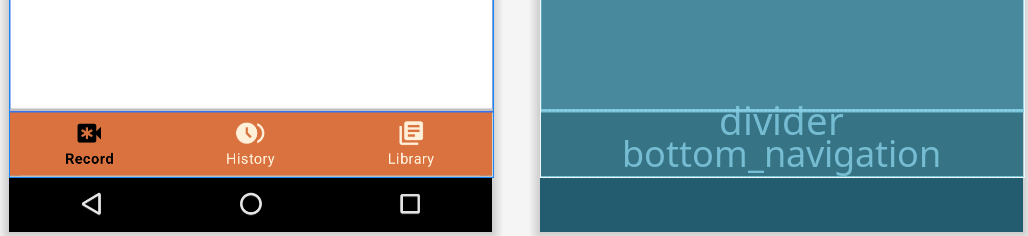
\includegraphics[width=2.9in]{src/navigation bottom.png}}
		\caption{Layout View of Specific Menu Design}
		\label{fig:nav_bottom}
	\end{figure}
	
	\begin{itemize}
		
		\item \textbf{User Interface (UI)}:
	    The UI for the Bottom Navigation is defined by two XML files: \texttt{activity\_main.xml} for the overall layout, including the BottomNavigationView as a container at the bottom of the app, and \texttt{menu/bottom\_navigation\_menu.xml} for the specific items within the navigation menu. In \texttt{activity\_main.xml}, a FrameLayout identified as \texttt{fragment\_container} serves as the placeholder for the various fragments switched by the Bottom Navigation. Below this, a BottomNavigationView widget is configured with parameters such as \texttt{itemIconTint} and \texttt{itemTextColor} to control the appearance of the navigation icons and text. This setup ensures a consistent and coherent visual representation across different fragments and contributes to the overall aesthetic and functional design of the navigation experience.
		
		\item \textbf{User Experience (UX)}:
		The Bottom Navigation is designed for ease of use, allowing users to seamlessly transition between the Record, History, and Library fragments by tapping on the corresponding icons in the navigation bar.
		
		\begin{figure}[htbp]
			\centerline{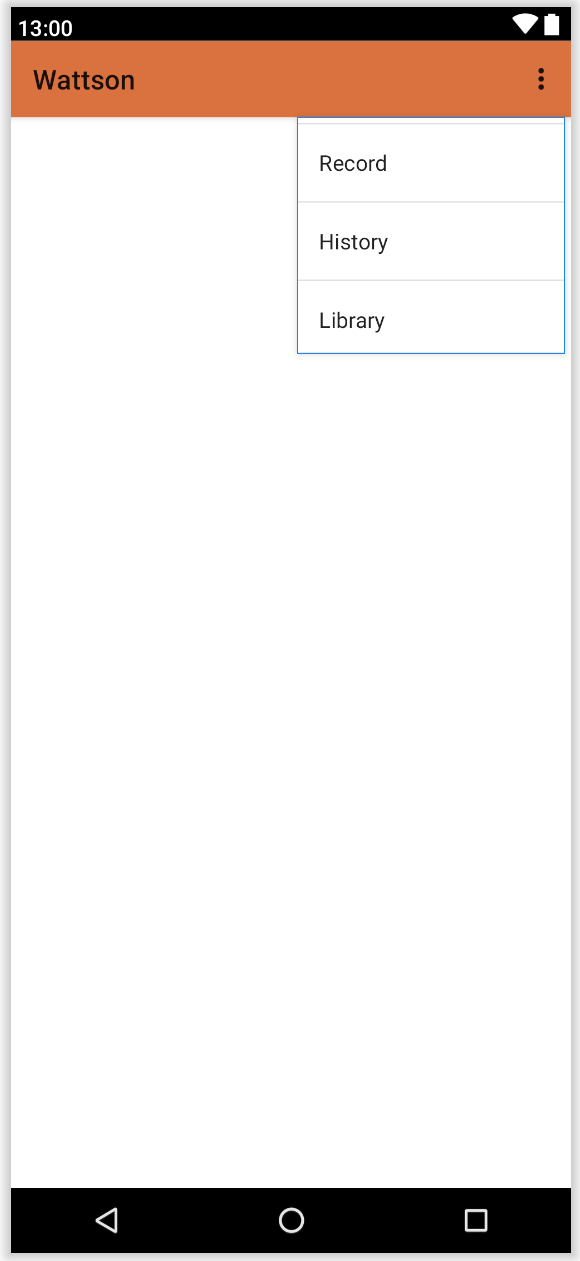
\includegraphics[width=1.7in]{src/menu.png}}
			\caption{Layout View of Bottom Navigation}
			\label{fig:menu}
		\end{figure}
		
		\item \textbf{Functionality Implementation}:
		The functionality of the Bottom Navigation is intricately designed within the \texttt{MainActivity} class of the app. Two pivotal methods, \texttt{navListener} and \texttt{switchFragment}, are central to its operation. The \texttt{navListener} is an instance of \texttt{navListener} and serves as the primary method for monitoring user interactions with the Bottom Navigation items. When an item is selected, this listener invokes the corresponding action, determined by the item's ID. Each ID is associated with one of the app's fragments; for instance, \texttt{R.id.navigation\_record} corresponds to the \texttt{RecordFragment}. The \texttt{navListener} ensures that the correct fragment is selected based on the user's choice, facilitating a responsive and interactive navigation experience. The \texttt{switchFragment} method is responsible for the dynamic and seamless replacement of fragments within the \texttt{fragment\_container}, which is defined in the \texttt{activity\_main.xml}. This method performs a fragment transaction, which is a series of steps to add, remove, or replace fragments in the activity's view hierarchy. Before switching, \texttt{switchFragment} checks if the current fragment is an instance of \texttt{RecordFragment} and, if so, stops any ongoing operations within it to reset the state. This is crucial to prevent any potential interference with the incoming fragment. After this check, the method executes the transaction to display the selected fragment. By managing these transitions, the method ensures that the user interface remains responsive and the transitions appear smooth to the user, thereby enhancing the overall user experience. In summary, these methods together form a robust navigation system that not only responds promptly to user input but also maintains the integrity and continuity of the user interface. This careful implementation underpins the app's navigation efficiency and contributes significantly to its usability.
		
		\begin{figure*}[ht]
			\centering
			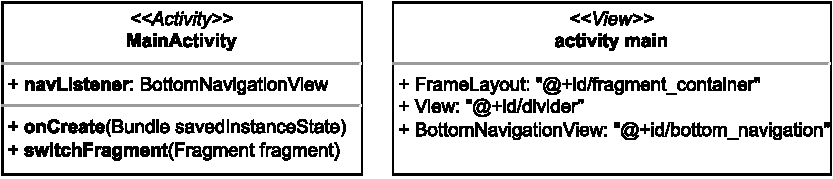
\includegraphics[width=5in]{src/main activity.pdf}
			\caption{Classes Diagram of Bottom Navigation Part}
			\label{fig:main_class}
		\end{figure*}
		
		\item \textbf{Performance Considerations}:
		The performance of the Bottom Navigation is a critical aspect of the app's overall user experience. Fast and efficient fragment transitions are imperative to maintain a fluid interaction. The app is designed to minimize the load times and resource usage when switching between different sections, ensuring that the user can navigate the app with minimal latency.
	\end{itemize}
	
	\begin{table*}[b]
		\centering
		\begin{tabularx}{6.2in}{|X|X|X|X|X|}
			\hline
			\textbf{Event} & \textbf{Stage} & \textbf{\textit{Duration (ms)}} & \textbf{\textit{CPU Usage (\%)}} & \textbf{\textit{Memory Usage (MB)}} \\ \hline
			Touch Event Press & Switch Fragment  & \textit{100.18}  & \textit{\textless 1}            & \textit{10.4} \\ \hline
		\end{tabularx}
		\caption{Performance Metrics for Bottom Navigation Part}
		\label{tab:nav_performance}
	\end{table*}
	
	\subsection{Database Management Part}
	
	The Database Management component is vital for the app's functionality, handling the storage, retrieval, and processing of user and application data.
	
	\begin{itemize}
		\item \textbf{Permissions and Data Management}:
		The class of \texttt{DatabaseHelper} encapsulates the complexity of database creation, upgrade, and data management within the app. In Android, SQLite databases are inherently private to the application, which means that no special permissions are required for an app to read from or write to the databases it creates. This class leverages this architecture to handle data within the confines of the app's secure storage without necessitating explicit user permissions, thus simplifying the data management process.
		
		\begin{figure}[htbp]
			\centerline{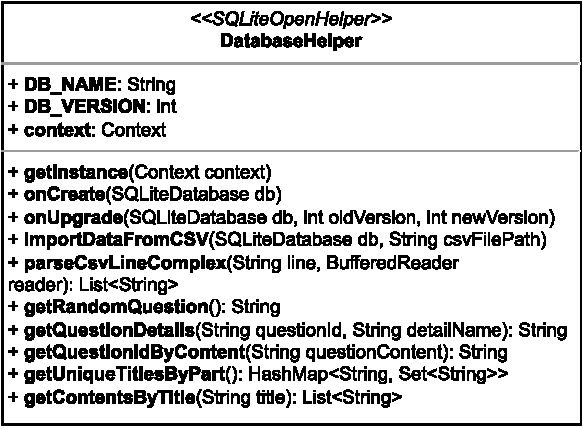
\includegraphics[width=2.8in]{src/datahelper.pdf}}
			\caption{Class of DataHelper}
			\label{fig:datahelper class}
		\end{figure}
		
		When the \texttt{DatabaseHelper} is instantiated, it either creates a new database if it does not exist or opens an existing one for reading and writing purposes. The class implements the \texttt{SQLiteOpenHelper} interface, which provides a framework for managing database creation and version management.  SQLite's role within the Android ecosystem is pivotal. It is a lightweight, file-based database management system that's integrated into Android, making it an ideal choice for mobile applications that require a robust data storage solution without the overhead of a full-fledged database server. SQLite supports standard SQL syntax and is highly optimized for performance on mobile devices, providing mechanisms such as transactions to maintain database integrity even when operations are interrupted. The \texttt{DatabaseHelper} class ensures that all database interactions are performed efficiently and correctly. It manages the flow of data to and from the database, encapsulating the complexities of raw SQL handling. 
		
		\begin{itemize}
			\item \texttt{onUpgrade} method facilitates the transition to new database versions, preserving data integrity and consistency across app updates.
			
			\item  \texttt{onCreate} method is only called when the database is created for the first time, ensuring that the schema is set up correctly. 
			
			\item \texttt{getWritableDatabase} and \texttt{getReadableDatabase}, it abstracts the underlying SQLite operations, providing a high-level interface for other components of the app to interact with the database. This approach guarantees data integrity and the security of the stored data, as SQLite enforces strict typing and transactional integrity, making the database resistant to corruption and ensuring the atomicity of operations.
		\end{itemize}
		
		Furthermore, the class employs best practices such as prepared statements and batch insertions to enhance performance and protect against SQL injection attacks. These measures are crucial for maintaining the security of the app's data and providing a seamless and responsive user experience.
		
		\item \textbf{Error Handling and User Feedback}:
		The class includes comprehensive error handling to cope with potential database access issues or data retrieval problems. It uses logging mechanisms, as seen with the \texttt{Log.e} calls, to notify developers of issues that occur during database operations. User feedback mechanisms are integrated into the app to inform users of any issues with data they are interacting with, providing a seamless experience.
		
		\item \textbf{Functionality Implementation}:
		\texttt{DatabaseHelper} class is endowed with several pivotal methods that facilitate various aspects of data manipulation and retrieval, crucial for the app's dynamic content management:
		
		\begin{itemize}
			\item \texttt{getRandomQuestion()} method showcases the use of SQLite's \texttt{RANDOM()} function to fetch a random entry from the questions table. This method enhances user engagement by providing varied content in scenarios such as quiz apps or practice tests where unpredictability is desired.
			
			\item \texttt{getQuestionDetails()} is tailored to retrieve specific details of a question, such as its type or content, based on a unique identifier. This function's precise data retrieval is essential for displaying question details or further processing within the app.
			
			\item \texttt{getQuestionIdByContent()} inversely maps a question's content to its unique ID. This is particularly useful for functions like bookmarking or referencing questions where a stable identifier is necessary to recall specific records.
			
			\item \texttt{getUniqueTitlesByPart()} compiles a list of unique titles for each part of the app's content, using a \texttt{HashMap} to ensure that each part is associated with a distinct set of titles. This method aids in categorizing content, making navigation and organization within the app more intuitive and efficient.
		\end{itemize}
		The initial population of the database with data from a CSV file during the creation phase is handled methodically. The \texttt{importDataFromCSV()} function reads the CSV file line by line, parsing each line into individual columns, and inserts the data into the SQLite database using prepared statements. This process not only pre-populates the app with a rich dataset but also showcases the utility of batch processing in database operations for enhanced performance. These methods collectively underscore the sophisticated data handling capabilities of the \texttt{DatabaseHelper} class. By abstracting the complexities of raw SQL queries and database interactions, the class provides a streamlined and efficient mechanism for data querying, insertion, and updates. This functionality is paramount in maintaining the responsiveness and dynamism of the app, allowing it to serve up-to-date content to the user with minimal delay and ensuring a smooth user experience.
		
		\item \textbf{Performance Considerations}:
		The performance of database operations is a key concern for the app's overall responsiveness. \texttt{DatabaseHelper} is optimized to handle data-intensive operations with minimal performance overhead. The use of transactions during CSV import and prepared statements for database insertion help to reduce the time taken for bulk data operations. Furthermore, the class is designed as a singleton to prevent unnecessary database connections, which can significantly impact performance. The methods are also optimized to ensure that database queries are executed quickly and efficiently, providing fast access to data when needed by the app.
	\end{itemize}

	\section{Evaluation}
	\subsection{Challenges}
	During the development of our application, several significant challenges were encountered, ranging from engineering complexities to user interface design concerns. These challenges were critical to address as they significantly impacted the overall functionality and user experience of the application. The key challenges included:
	
	\begin{enumerate}
		\item A major engineering challenge was managing the lifecycle of \texttt{RecorderMedia} and \texttt{PlayMedia}. These components are essential in Android app development for handling audio recording and playback. The challenge lay in accurately implementing their opening and closing mechanisms. Inadequate management of these resources could lead to application crashes, undermining stability and reliability.
		
		\item Designing the layout for \texttt{HistoryFragment} and \texttt{LibraryFragment} posed another significant challenge. We deliberated extensively over the choice of the ViewGroup to use, comparing \texttt{LinearLayout}, \texttt{FrameLayout}, and \texttt{GridView}. Our goal was to achieve an expandable view upon clicking, but these options did not fully meet our requirements.
		
		\newpage
		\item The design of the navigation bottom posed a challenge as we initially considered using activity transitions to switch views. However, this approach was found to be resource-intensive and resulted in unnatural transitions, even when animations were removed using the \texttt{no\_animation} method.
	\end{enumerate}
	
	\subsection{Solutions}
	To overcome these challenges, we implemented a series of solutions that enhanced both the functionality and user experience of our application:
	
	\begin{enumerate}
		\item To tackle the first challenge, we utilized \texttt{Log} and \texttt{Toast} messages during development for real-time situational assessment. We also established an \texttt{AudioManager} object to manage \texttt{RecorderMedia} and \texttt{PlayMedia} effectively. The use of dedicated \texttt{Recording} objects for sound management further ensured efficient resource utilization, resolving stability issues.
		
		\item For the layout design challenge in \texttt{HistoryFragment} and \texttt{LibraryFragment}, we discovered that newer versions of Android API support \texttt{ExpandableListView}. This necessitated the use of a \texttt{CustomExpandableListAdapter} for efficient management. \texttt{ExpandableListView} allowed us to achieve the desired expandable effect upon user interaction, which was crucial for our app’s design.
		
		\item To address the navigation issue, we transitioned from using separate activities to implementing fragments. This was achieved through a \texttt{OnNavigationItemSelectedListener} and a \texttt{switchFragment(Fragment fragment)} method. This approach not only reduced resource consumption but also provided smoother and more natural transitions between different parts of the app.
	\end{enumerate}
	
	\subsection{HCI}
	In terms of Human-Computer Interaction, careful consideration was given to the app's usability. For the \texttt{Tap to record} feature, the lower third of the screen was chosen for interaction, as this area is most easily accessible with the thumb, making it convenient for users. This design allows users to start, pause, resume, and stop recording effortlessly, which is highly beneficial for concentrating on their oral practice without the need to constantly look at the phone. After recording, the interface efficiently uses three ImageButtons to execute different functions, making the app more intuitive and user-friendly.
	
	\subsection{Functionality and Integration}
	Regarding the question of whether the features of our app work as intended and their synergy with other features, the Record Part has been successfully implemented and integrates well with the overall functionality of the app. However, due to the solo nature of the development process and academic pressures, including language exams and assignments, two features could not be completed in time. These are the manual note-taking feature and the implementation of voice-to-text conversion using Android's native APIs.
	
	\subsection{Future Enhancements and Reworked Design}
	Given more time and resources, several enhancements and reworks are envisioned for the app. Keeping in mind the lecture on context awareness, the following improvements are proposed:
	\begin{enumerate}
		\item \textbf{Enhanced Context Awareness:} Incorporating more advanced context-aware features, such as adjusting the difficulty level of questions based on the user's proficiency and learning pace, would make the app more responsive to individual needs.
		
		\item \textbf{Interactive Note-Taking Feature:} As previously mentioned, the manual note-taking feature was not completed. With additional time, this feature would be implemented to allow users to jot down notes or key points during their practice sessions, enhancing the learning experience.
		\item \textbf{Voice-to-Text Functionality:} Implementing the voice-to-text feature using Android's APIs would allow users to see a transcription of their spoken responses, aiding in self-assessment and improvement.
		\item \textbf{UI/UX Rework:} Based on user feedback and HCI principles, the user interface and experience could be further refined. This might include simplifying navigation, making the app more intuitive, and enhancing visual appeal to keep users engaged.
	\end{enumerate}
	
	These proposed enhancements and redesigns are aimed at making the app not only more user-friendly but also more effective as a language learning tool, leveraging the potential of technology to provide a personalized and engaging learning experience.
	
	\section{Conclusion}
	In conclusion, I successfully navigated through key issues in engineering and interface design, implementing effective solutions that have significantly improved the app's performance and usability. My focus on human-computer interaction principles has resulted in an intuitive and accessible tool for IELTS speaking practice. Wattson stands as a testament to the effectiveness of thoughtful design and user-centered development in creating applications that are not only functional but also user-friendly. I believe that this app will make a substantial difference in assisting users in their language learning journey.
	
	\begin{thebibliography}{00}
		\bibitem{b1} Google Developers, ``Documentation | Android Developers,'' available at \url{https://developer.android.com/guide}
		
		\bibitem{b2} Android Developers, ``View | Android Developers,'' available at \url{https://developer.android.com/reference/classes}
		
		\bibitem{b3} Android Open Source Project, ``Android OS Source Documentation | Android Open Source Project,'' available at \url{https://source.android.com/docs}
		
		\bibitem{b4} Android Developers, ``Services overview | Background work | Android Developers,'' available at \url{https://developer.android.com/guide/components/services}
		
	\end{thebibliography}
	
	\newpage
	\appendix
	\section{Appendix}
	\subsection{Project Repository}
	The source code and additional resources for this project are available in the GitHub repository at the following URL:
	
	\href{https://github.com/jonlai211/Wattson}{\textcolor{blue}{\uline{https://github.com/jonlai211/Wattson}}}
	
	\subsection{Shortcuts}
	\begin{figure}[htbp]
		\centerline{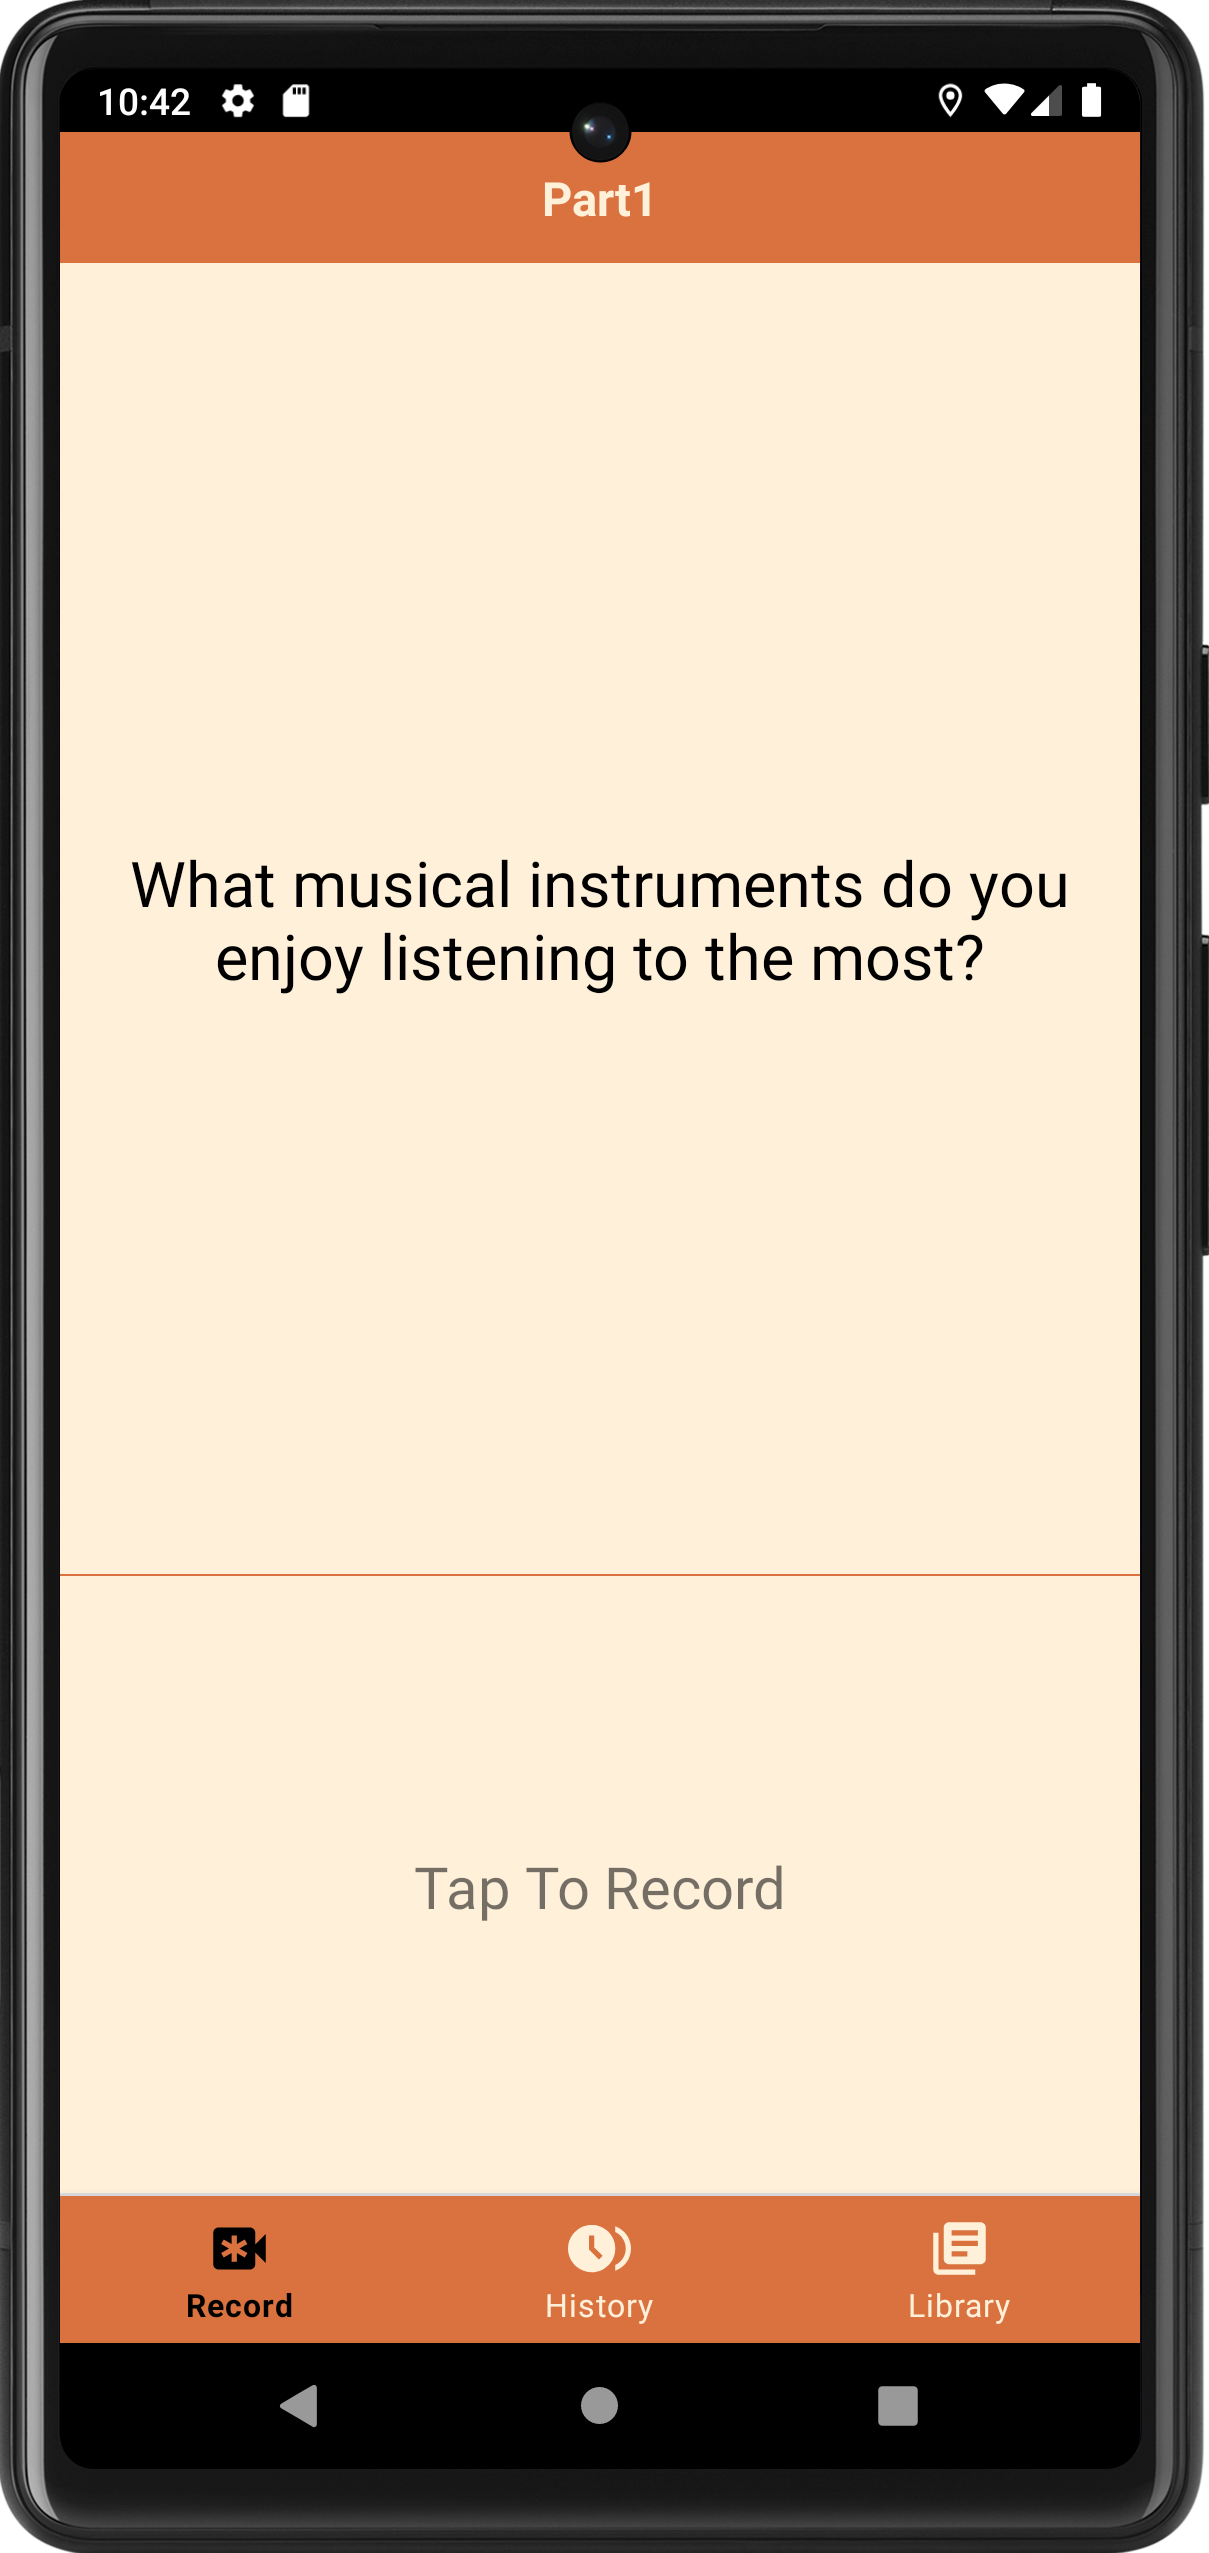
\includegraphics[height=3.5in]{src/record shortcut.png}}
		\caption{Record Shortcut}
		\label{fig:record_shortcut}
	\end{figure}
	
	\begin{figure}[htbp]
		\centerline{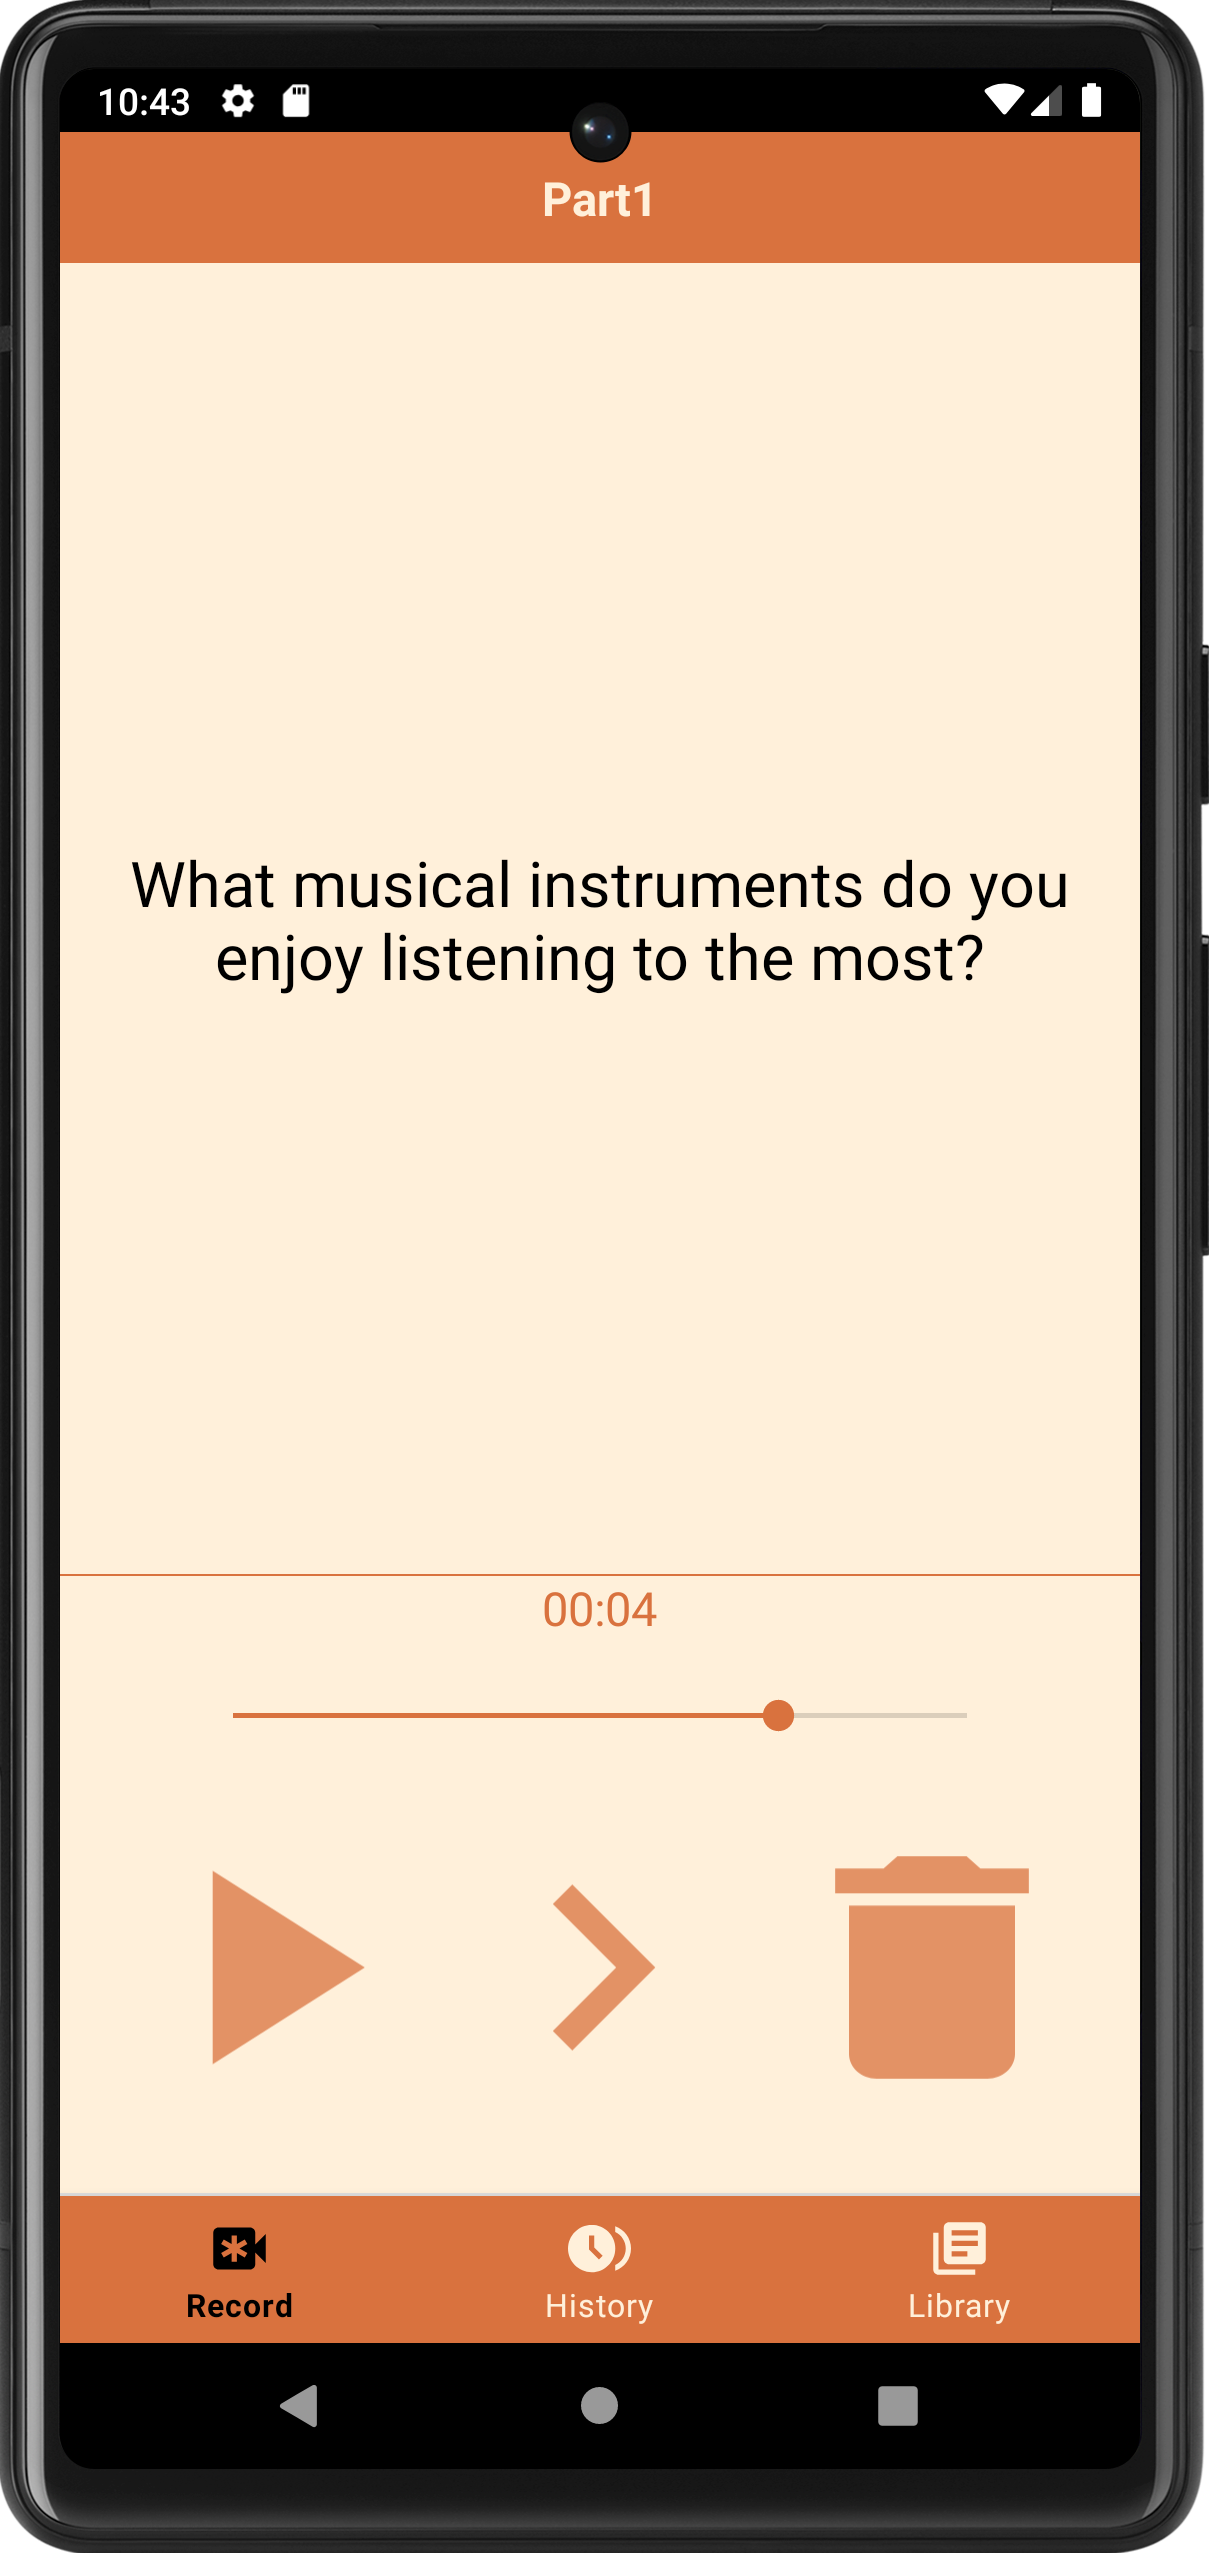
\includegraphics[height=3.5in]{src/control shortcut.png}}
		\caption{Control Shortcut}
		\label{fig:control_shortcut}
	\end{figure}
	
	\begin{figure}[htbp]
		\centerline{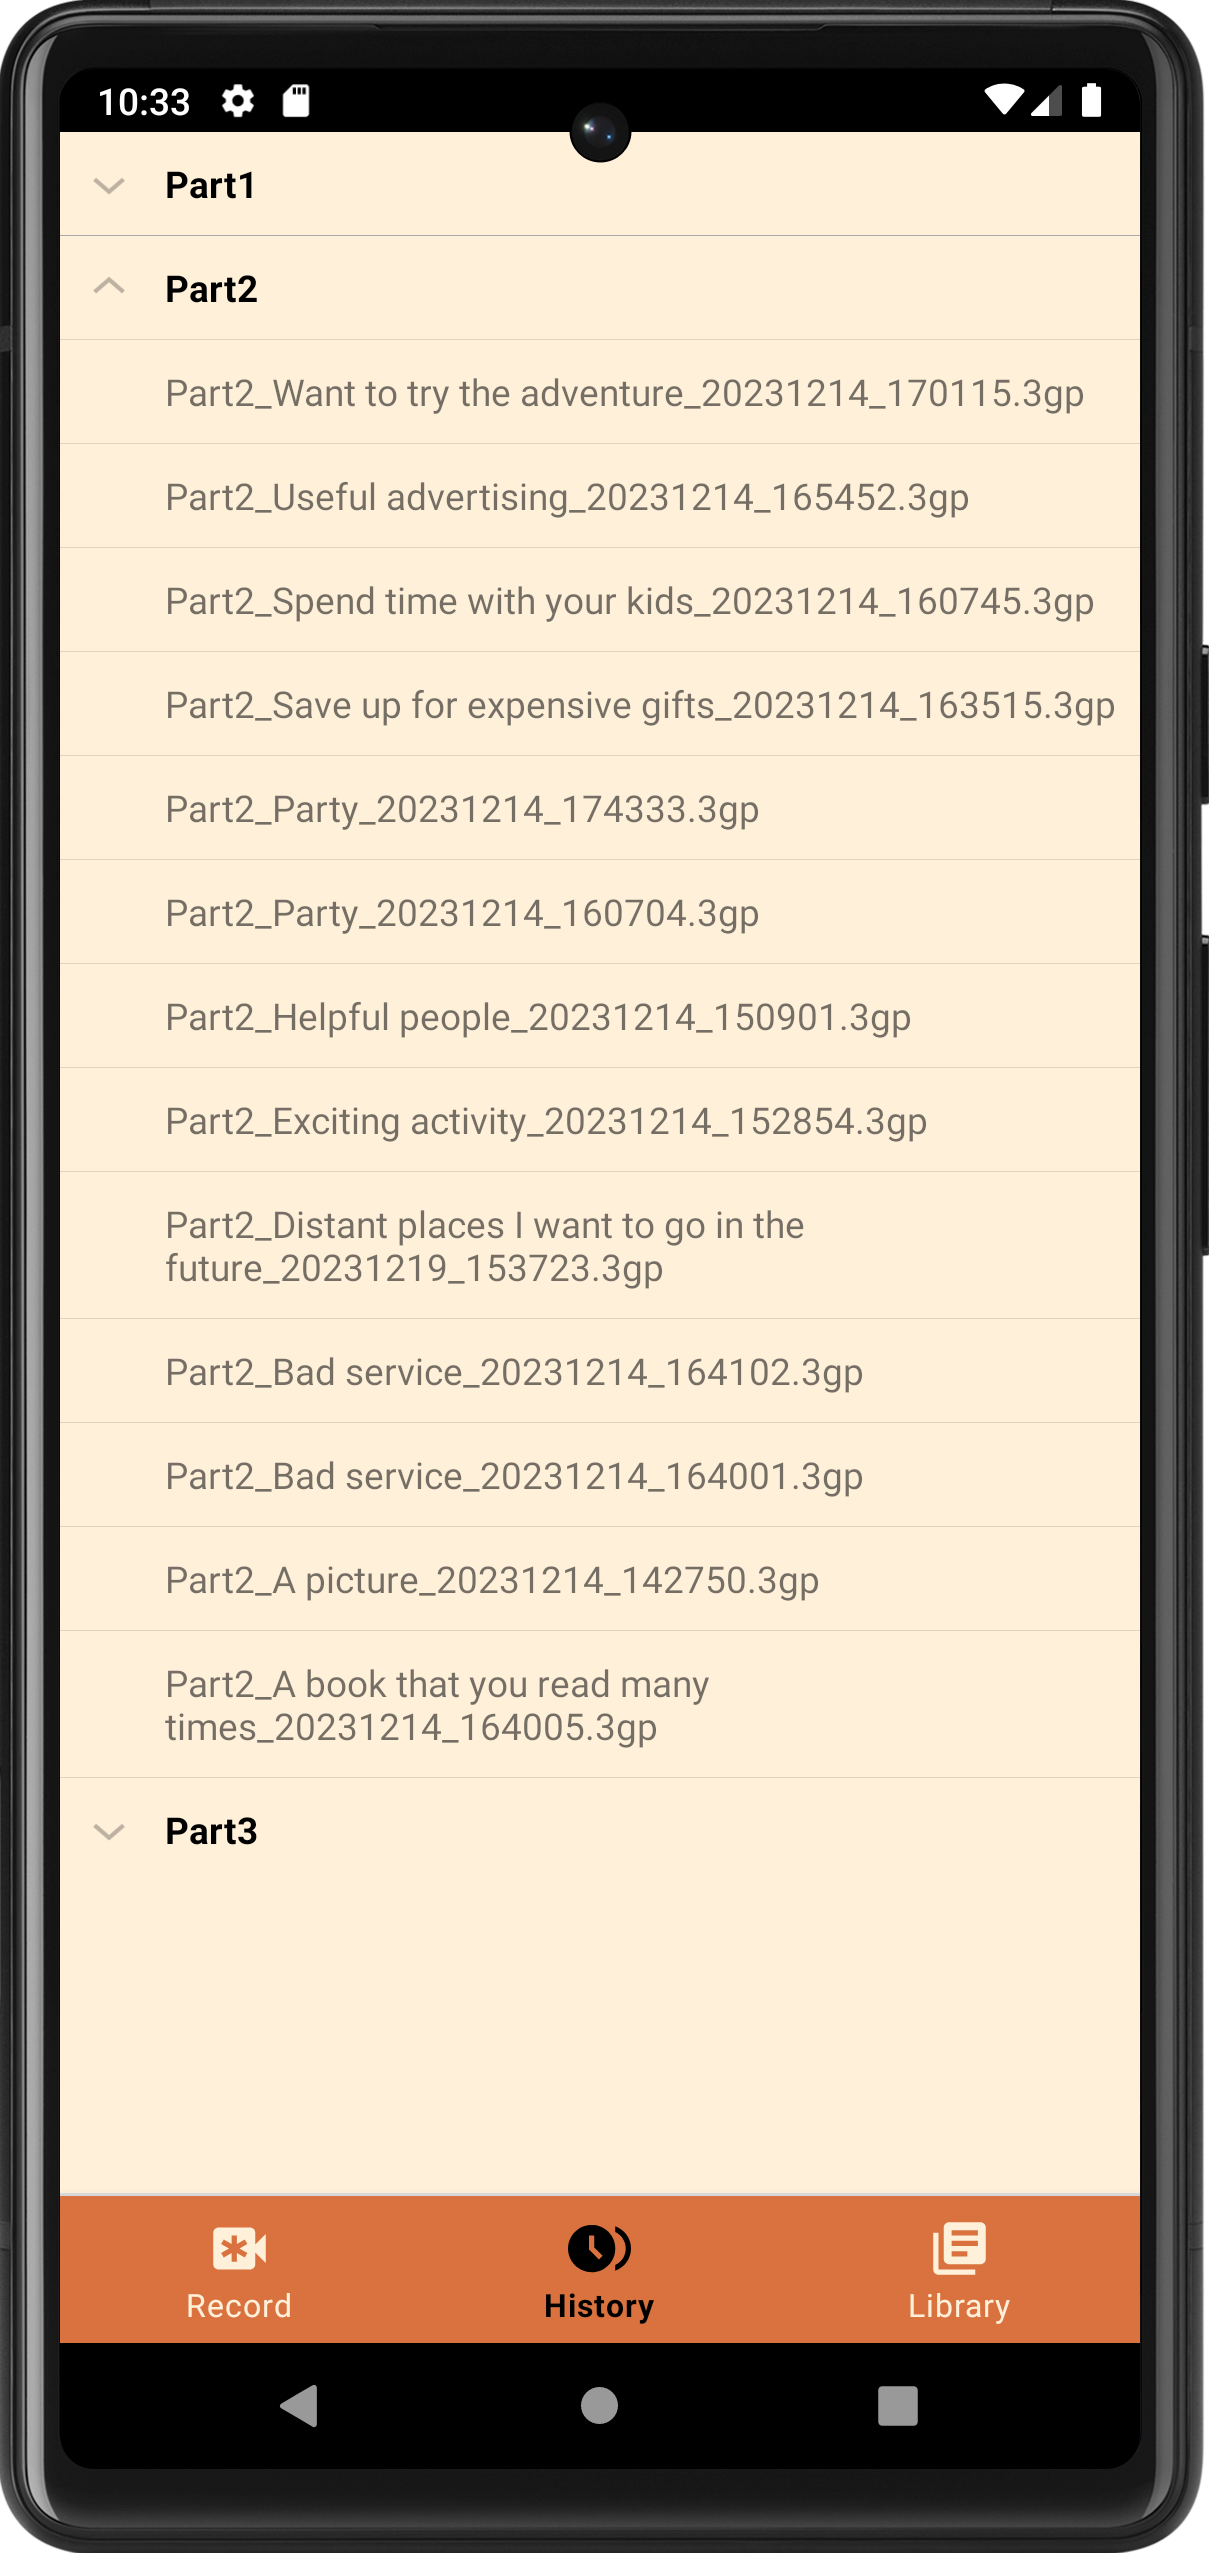
\includegraphics[height=3.5in]{src/history shortcut.png}}
		\caption{History Shortcut}
		\label{fig:history_shortcut}
	\end{figure}
	
	\begin{figure}[htbp]
		\centerline{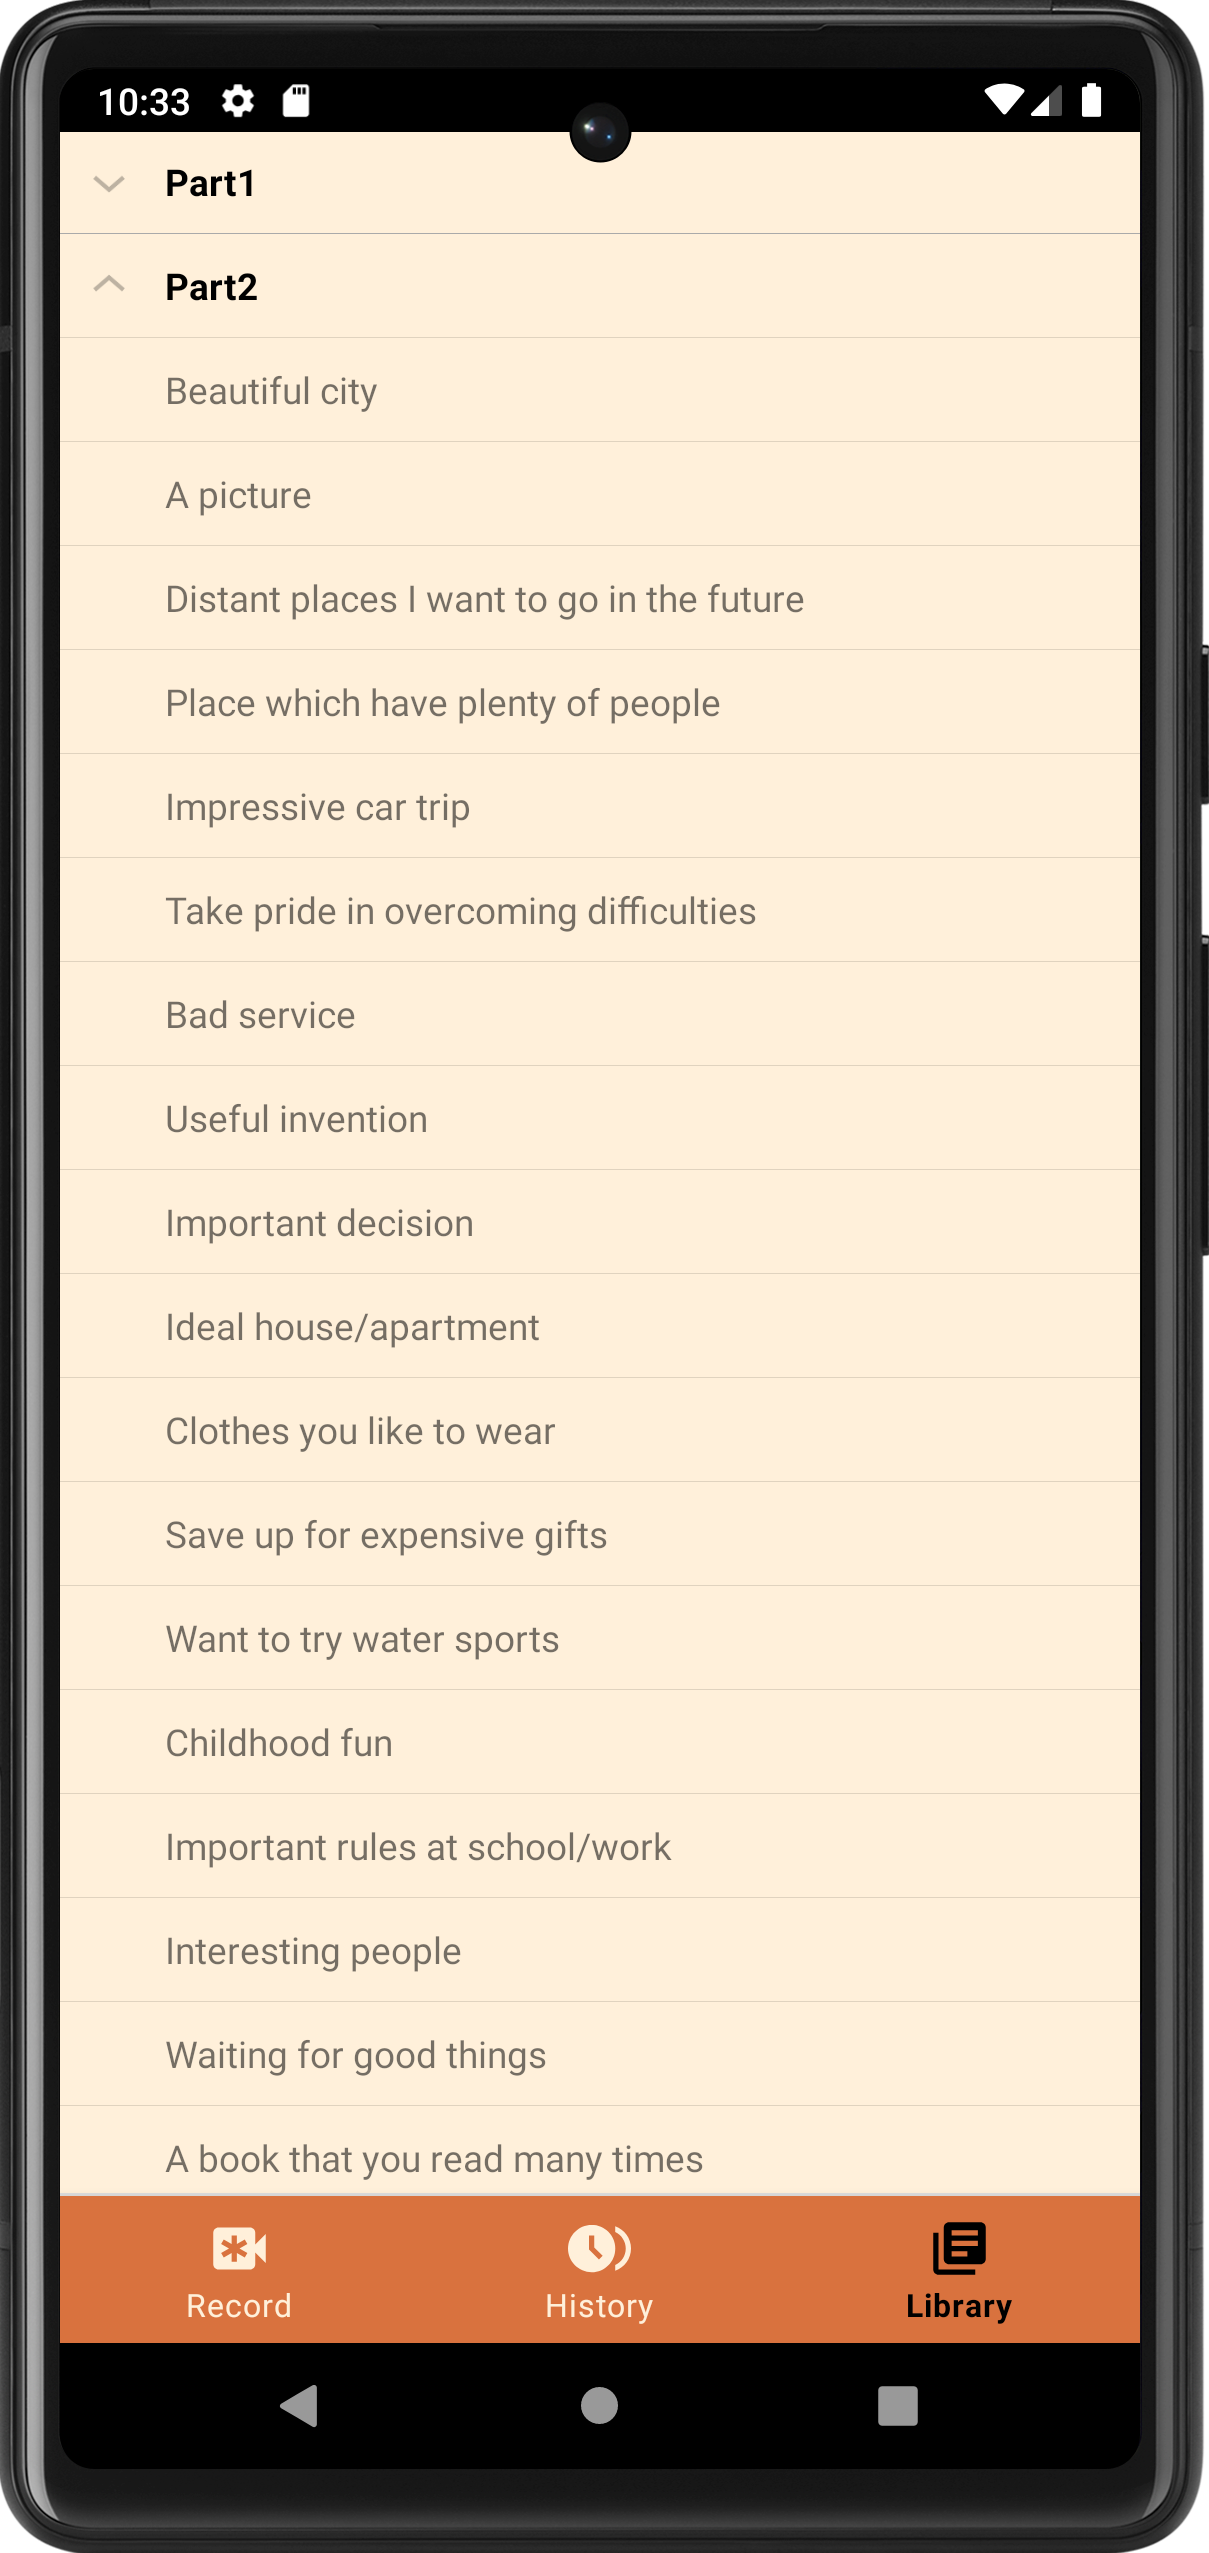
\includegraphics[height=3.5in]{src/library shortcut.png}}
		\caption{Library Shortcut}
		\label{fig:library_shortcut}
	\end{figure}
	
\end{document}
